\section{Result of the counting experiment}
The distribution of the dilepton invariant mass in the central and forward signal regions are shown in Figure~\ref{fig:resultsCC}. The resulting event yields are compared to the expectation from SM backgrounds in Table~\ref{tab:METresults2012}. A maximum likelihood fit is performed in each region to find the best estimator for the for the difference of expected and observed yield. The significances of deviations of this difference from zero are evaluated using the profile likelihood ratio of the signal and signal+background hypothesis~\cite{HiggsTool1}. In general, the observed data is in agreement with the background estimation within about one standard deviation, except for the low-mass region in the central dilepton selection. Here the observed yield exceeds the expectation by $109^{+48}_{-49}$ events. The size of this excess corresponds to a significance of 2.2~$\sigma$.  
\begin{figure}[htbp]
\centering
\begin{minipage}[t]{0.49\textwidth}
  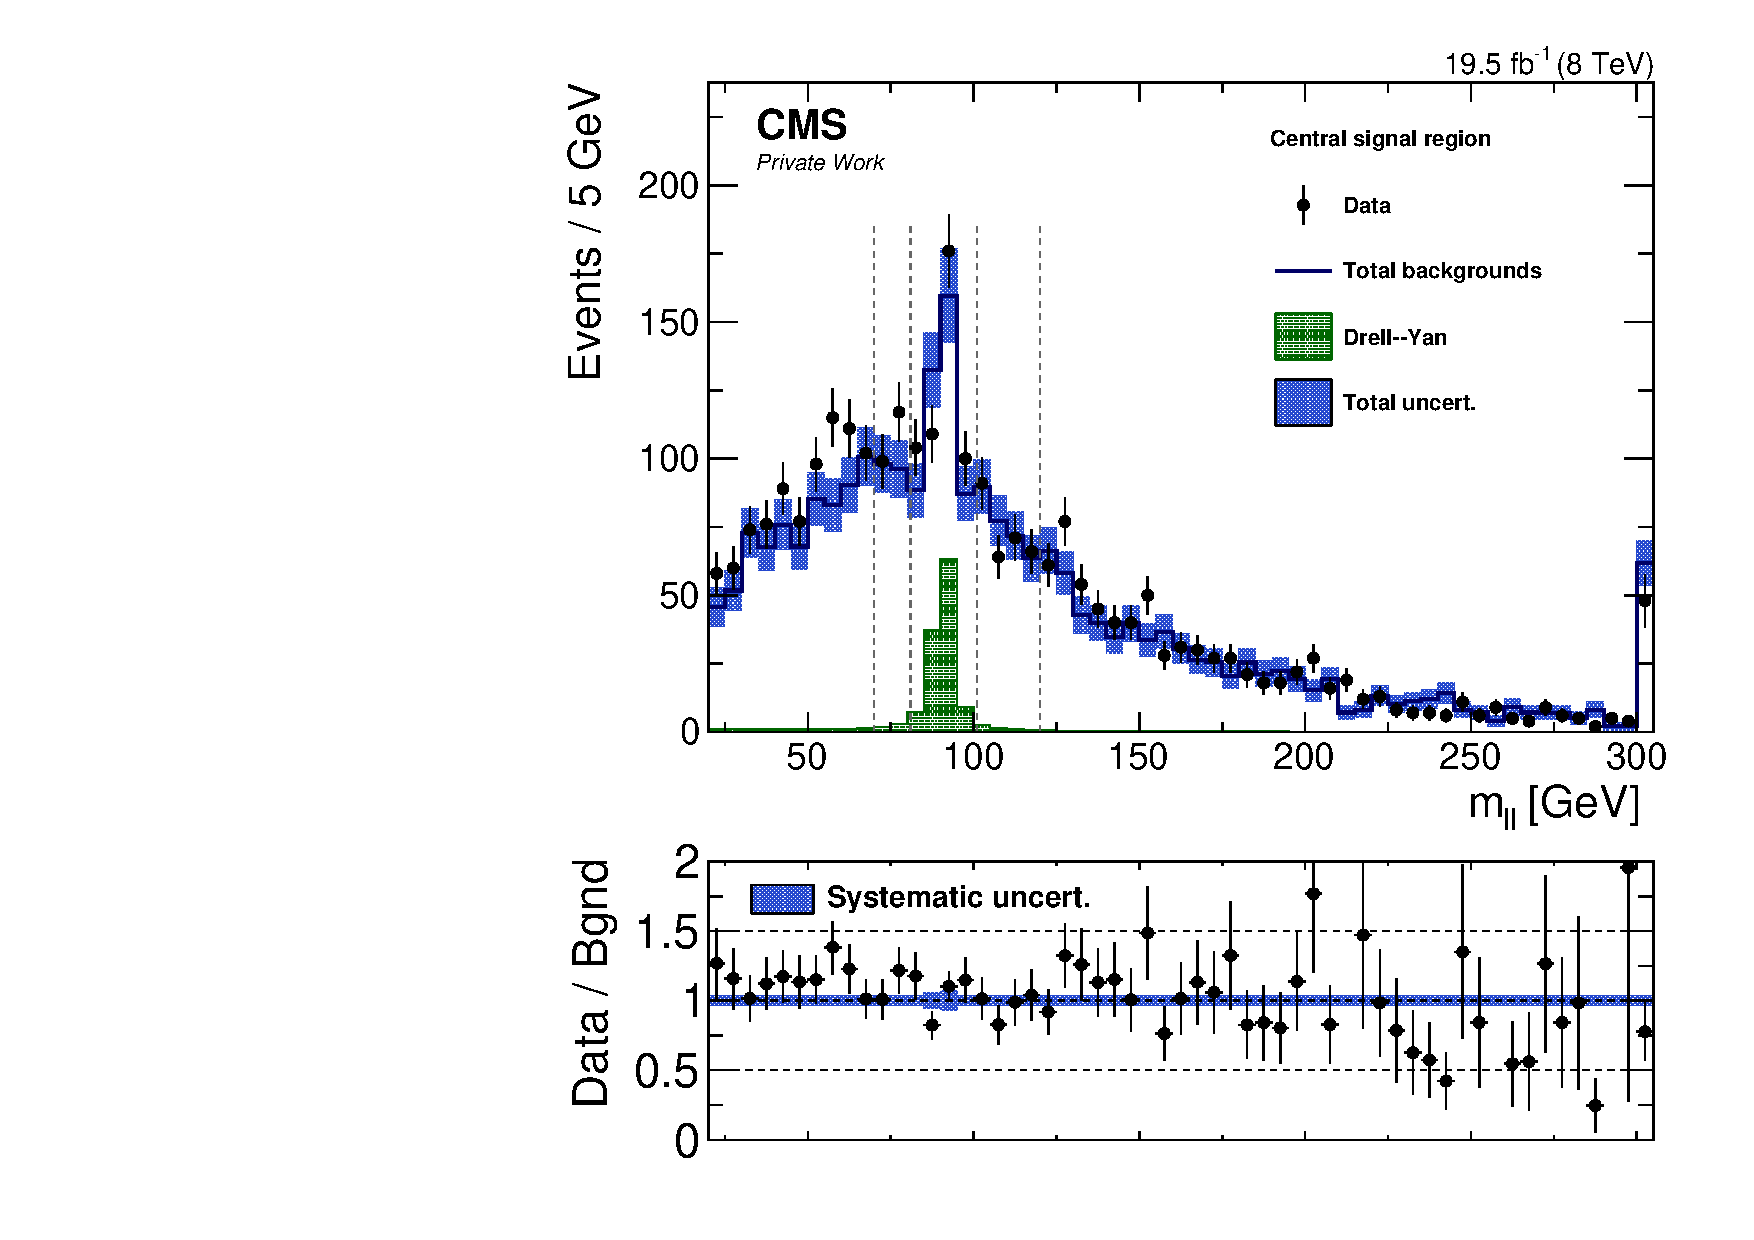
\includegraphics[width=\textwidth]{plots/results/mllResult_SignalCentral_Full2012_SF.pdf}
\end{minipage}
\begin{minipage}[t]{0.49\textwidth}
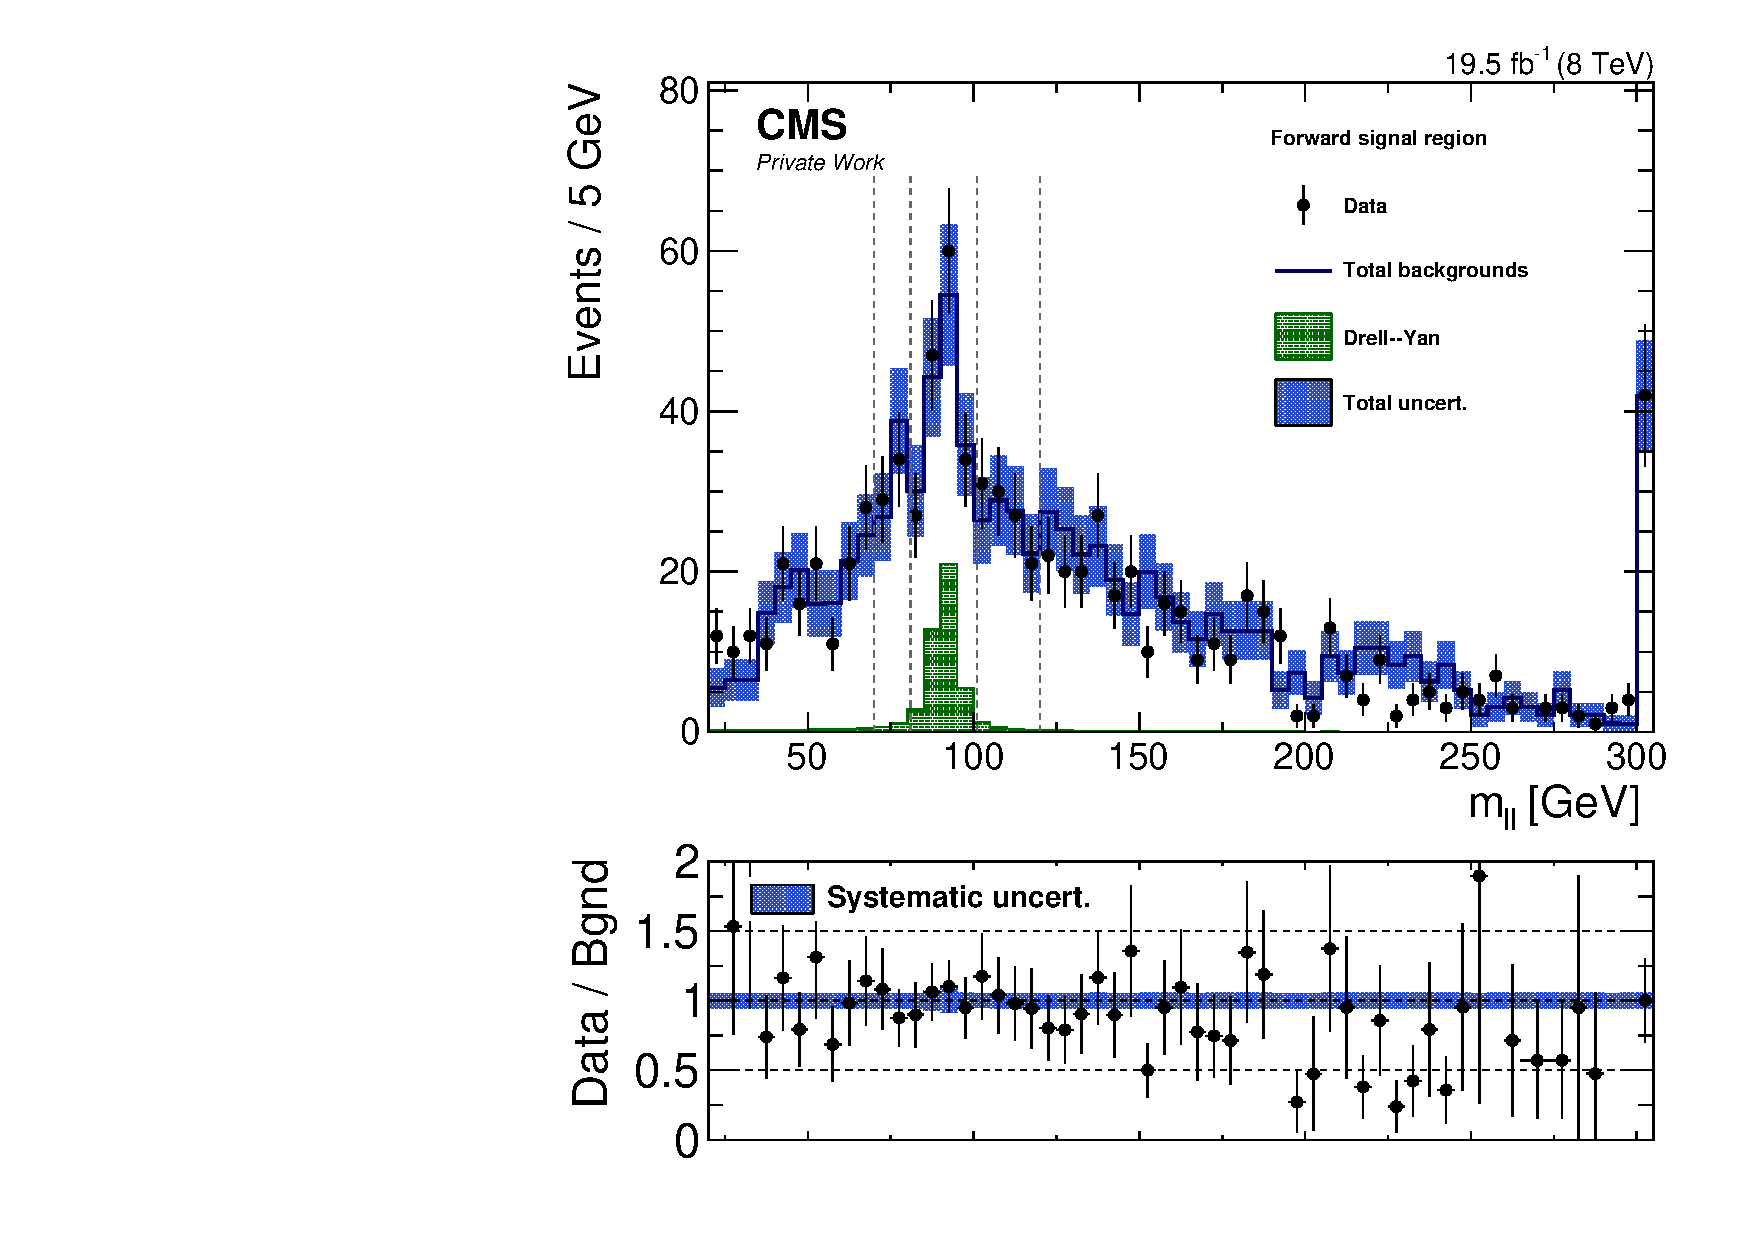
\includegraphics[width=\textwidth]{plots/results/mllResult_SignalForward_Full2012_SF.pdf}
\end{minipage}

\caption{Distribution of \mll in the signal region for the central (left) and forward (right) dilepton selection. The data is shown as black dots, while the total background prediction from data is shown as a blue histogram. The blue error bars indicate the combined statistical and systematic background uncertainty in each bin. The contribution from backgrounds containing a Z boson is shown as a green histogram. The dashed lines indicates the boundaries of the three mass bins. Beneath the plot the ratio of data to the background prediction is shown. The error bars include the statistical uncertainties of data and background, while the blue band indicates the systematic uncertainties on the background. }
\label{fig:resultsCC}
\end{figure} 


\begin{table}[btp]
 \renewcommand{\arraystretch}{1.3}
 \setlength{\belowcaptionskip}{6pt}
 \scriptsize
 \centering
 \caption{Results of the counting experiment in the six signal regions.
     The statistical and systematic uncertainties are added in quadrature, except for the flavor-symmetric backgrounds. The presented differences between the observed and estimated yields are obtained with a maximum likelihood fit (see text).    Low-mass refers to $20\GeV < \mll < 70$\GeV, on-\Z to  $81\GeV < \mll < 101$\GeV, and high-mass to $\mll > 120$\GeV.
     }
  \label{tab:METresults2012}
  \begin{tabular}{l| cc | cc | cc}

    							& \multicolumn{2}{c}{low-mass} & \multicolumn{2}{c}{on-\Z} & \multicolumn{2}{c}{high-mass} \\ 

    \hline
                                &  Central        & Forward  &  Central  & Forward   &  Central        & Forward \\ 

    \hline
        Observed       &  865                   & 154              &  494            &  176       &   849           &   381    \\

    \hline
        Flav.-sym.    & $746\pm27\pm26$        & $144\pm12\pm7$  &  $368\pm19\pm13$ & $137\pm11\pm7$ & $789\pm28\pm28$ & $411\pm20\pm21$ \\

            Drell--Yan          & $8.6\pm2.7$            & $2.6\pm0.8$      & $119\pm21$ & $43\pm9$ & $2.7\pm0.8$ & $1.2\pm0.4$ \\

    \hline
            Total est.          & $755\pm38$            & $147\pm14$      & $488\pm31$ & $180\pm16$ & $792\pm39$ & $413\pm30$ \\

    \hline
         Obs. - est.  & $109\pm48$      & $7\pm19$ & $6\pm38 $ & $-5\pm21$ & $57\pm50$ & $-32\pm37 $ \\ 

    \hline
   Significance      & 2.2~$\sigma$    &  0.4~$\sigma$  & 0.1~$\sigma$ & $<$0.1~$\sigma$ & 1.1~$\sigma$ & $<$0.1~$\sigma$ \\ 


  \end{tabular}
\end{table}



In the Tables~\ref{tab:METresults2012MM} and~\ref{tab:METresults2012EE}, the results are shown separately for \EE and \MM events. As expected from the fact that \rmue is larger than one, the yields in the \MM channel are slightly larger than in the \EE channel. For the flavour-symmetry backgrounds, and therefore also for the total background estimates and the difference of observation and estimation, the yields in the \EE and \MM channels to not exactly add up to those in the combined SF channel. \fixme{Reference explenation once written} 

\begin{table}[hbtp]
 \renewcommand{\arraystretch}{1.3}
 \setlength{\belowcaptionskip}{6pt}
 \scriptsize
 \centering
 \caption{Results of the counting experiment for \EE events only.
     The statistical and systematic uncertainties are added in quadrature, except for the flavor-symmetric backgrounds. The presented differences between the observed and estimated yields are obtained with a maximum likelihood fit (see text).    Low-mass refers to $20 < \mll < 70$\GeV, on-\Z to  $81 < \mll < 101$\GeV, and high-mass to $\mll > 120$\GeV.
     }
  \label{tab:METresults2012EE}
  \begin{tabular}{l| cc | cc | cc}

    							& \multicolumn{2}{c}{low-mass} & \multicolumn{2}{c}{on-\Z} & \multicolumn{2}{c}{high-mass} \\ 

    \hline
                                &  Central        & Forward  &  Central  & Forward   &  Central        & Forward \\ 

    \hline
        Observed       &  389                   & 53              &  232            &  86       &   401           &   195    \\

    \hline
        Flav.-sym.    & $337\pm12\pm19$        & $61\pm5\pm6$  &  $166\pm8\pm9$ & $58\pm5\pm5$ & $357\pm12\pm21$ & $175\pm8\pm17$ \\

            Drell--Yan          & $4.3\pm1.3$            & $1.2\pm0.4$      & $62\pm11$ & $21\pm5$ & $1.5\pm0.5$ & $0.7\pm0.2$ \\

    \hline
            Total est.          & $342\pm23$            & $62\pm8$      & $229\pm17$ & $79\pm9$ & $358\pm24$ & $175\pm19$ \\

    \hline
         Obs. - est.  & $47\pm25$      & $-10\pm9$ & $3\pm21 $ & $6\pm12$ & $42\pm26$ & $19\pm18 $ \\ 

    \hline
   Significance      & 1.9~$\sigma$    &  $<$0.1~$\sigma$  & 0.1~$\sigma$ & 0.5~$\sigma$ & 1.7~$\sigma$ & 1.1~$\sigma$ \\ 


  \end{tabular}
\end{table}





\begin{table}[hbtp]
 \renewcommand{\arraystretch}{1.3}
 \setlength{\belowcaptionskip}{6pt}
 \scriptsize
 \centering
 \caption{Results of the counting experiment for \MM events only.
     The statistical and systematic uncertainties are added in quadrature, except for the flavor-symmetric backgrounds.
     Low-mass refers to $20 < \mll < 70$\GeV, on-\Z to  $81 < \mll < 101$\GeV and high-mass to $\mll > 120$\GeV.
     }
  \label{tab:METresults2012MM}
  \begin{tabular}{l| cc | cc | cc}

    							& \multicolumn{2}{c}{low-mass} & \multicolumn{2}{c}{on-\Z} & \multicolumn{2}{c}{high-mass} \\ 

    \hline
                                &  Central        & Forward  &  Central  & Forward   &  Central        & Forward \\ 

    \hline
        Observed       &  476                   & 101              &  262            &  90       &   448           &   186    \\

    \hline
        Flavor-symmetric    & $405\pm14\pm21$        & $79\pm6\pm6$  &  $200\pm10\pm10$ & $74\pm6\pm6$ & $428\pm15\pm23$ & $224\pm11\pm19$ \\

            Drell--Yan          & $4.4\pm1.4$            & $1.6\pm0.6$      & $58\pm10$ & $25\pm6$ & $1.2\pm0.4$ & $0.7\pm0.2$ \\

    \hline
            Total estimated          & $409\pm26$            & $80\pm9$      & $258\pm18$ & $100\pm11$ & $429\pm27$ & $225\pm22$ \\

    \hline
         Observed - estimated  & $67^{+29}_{-29}$      & $20^{+13}_{-13}$ & $3^{+22}_{-23} $ & $-11^{+13}_{-13}$ & $19^{+29}_{-29}$ & $-40^{+21}_{-21} $ \\ 

    \hline
   Significance      & 2.3~$\sigma$    &  1.6~$\sigma$  & 0.2~$\sigma$ & $<$0.1~$\sigma$ & 0.6~$\sigma$ & $<$0.1~$\sigma$ \\ 


  \end{tabular}
\end{table}







\begin{figure}[htbp]
\centering
\begin{minipage}[t]{0.49\textwidth}
  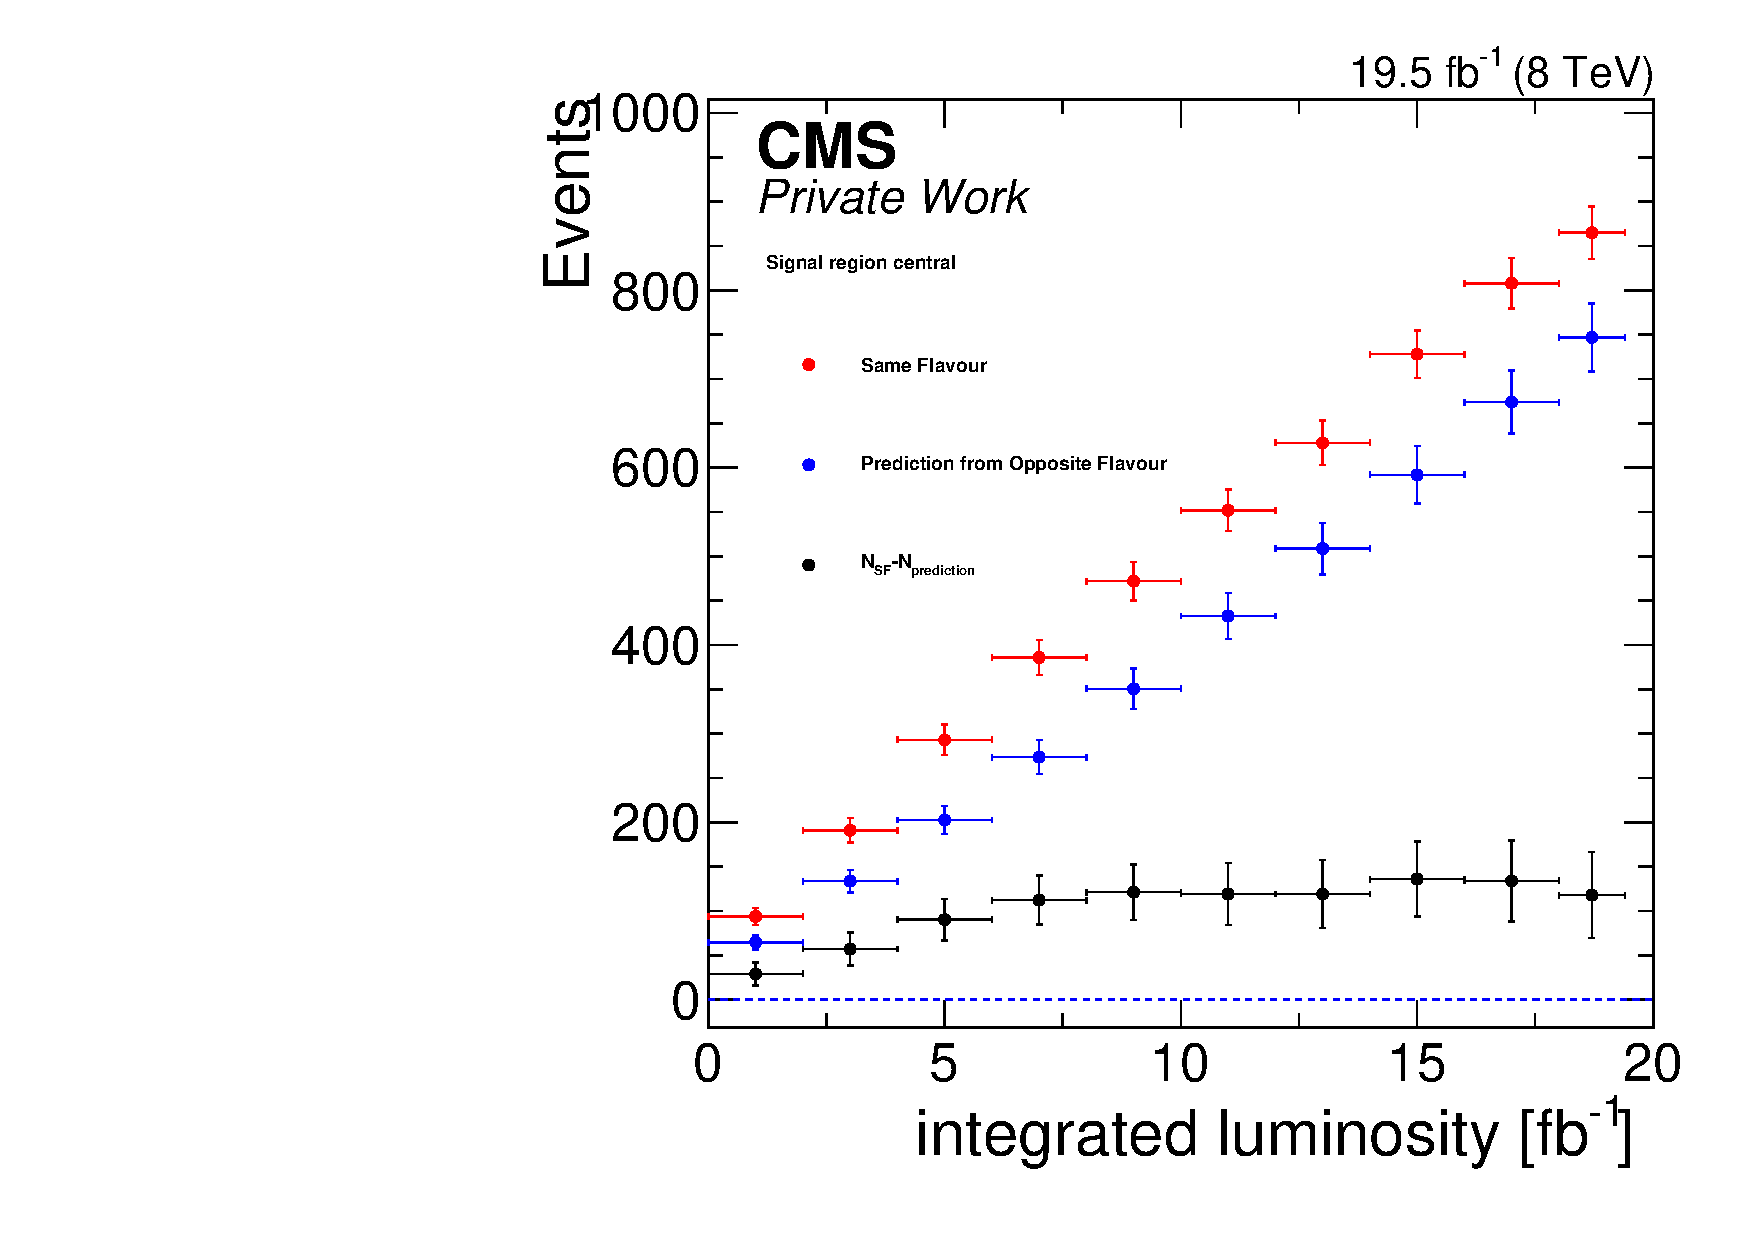
\includegraphics[width=\textwidth]{plots/results/YieldvsLumi_SignalCentral_Mll_edgeMassFull2012.pdf}
\end{minipage}
\begin{minipage}[t]{0.49\textwidth}
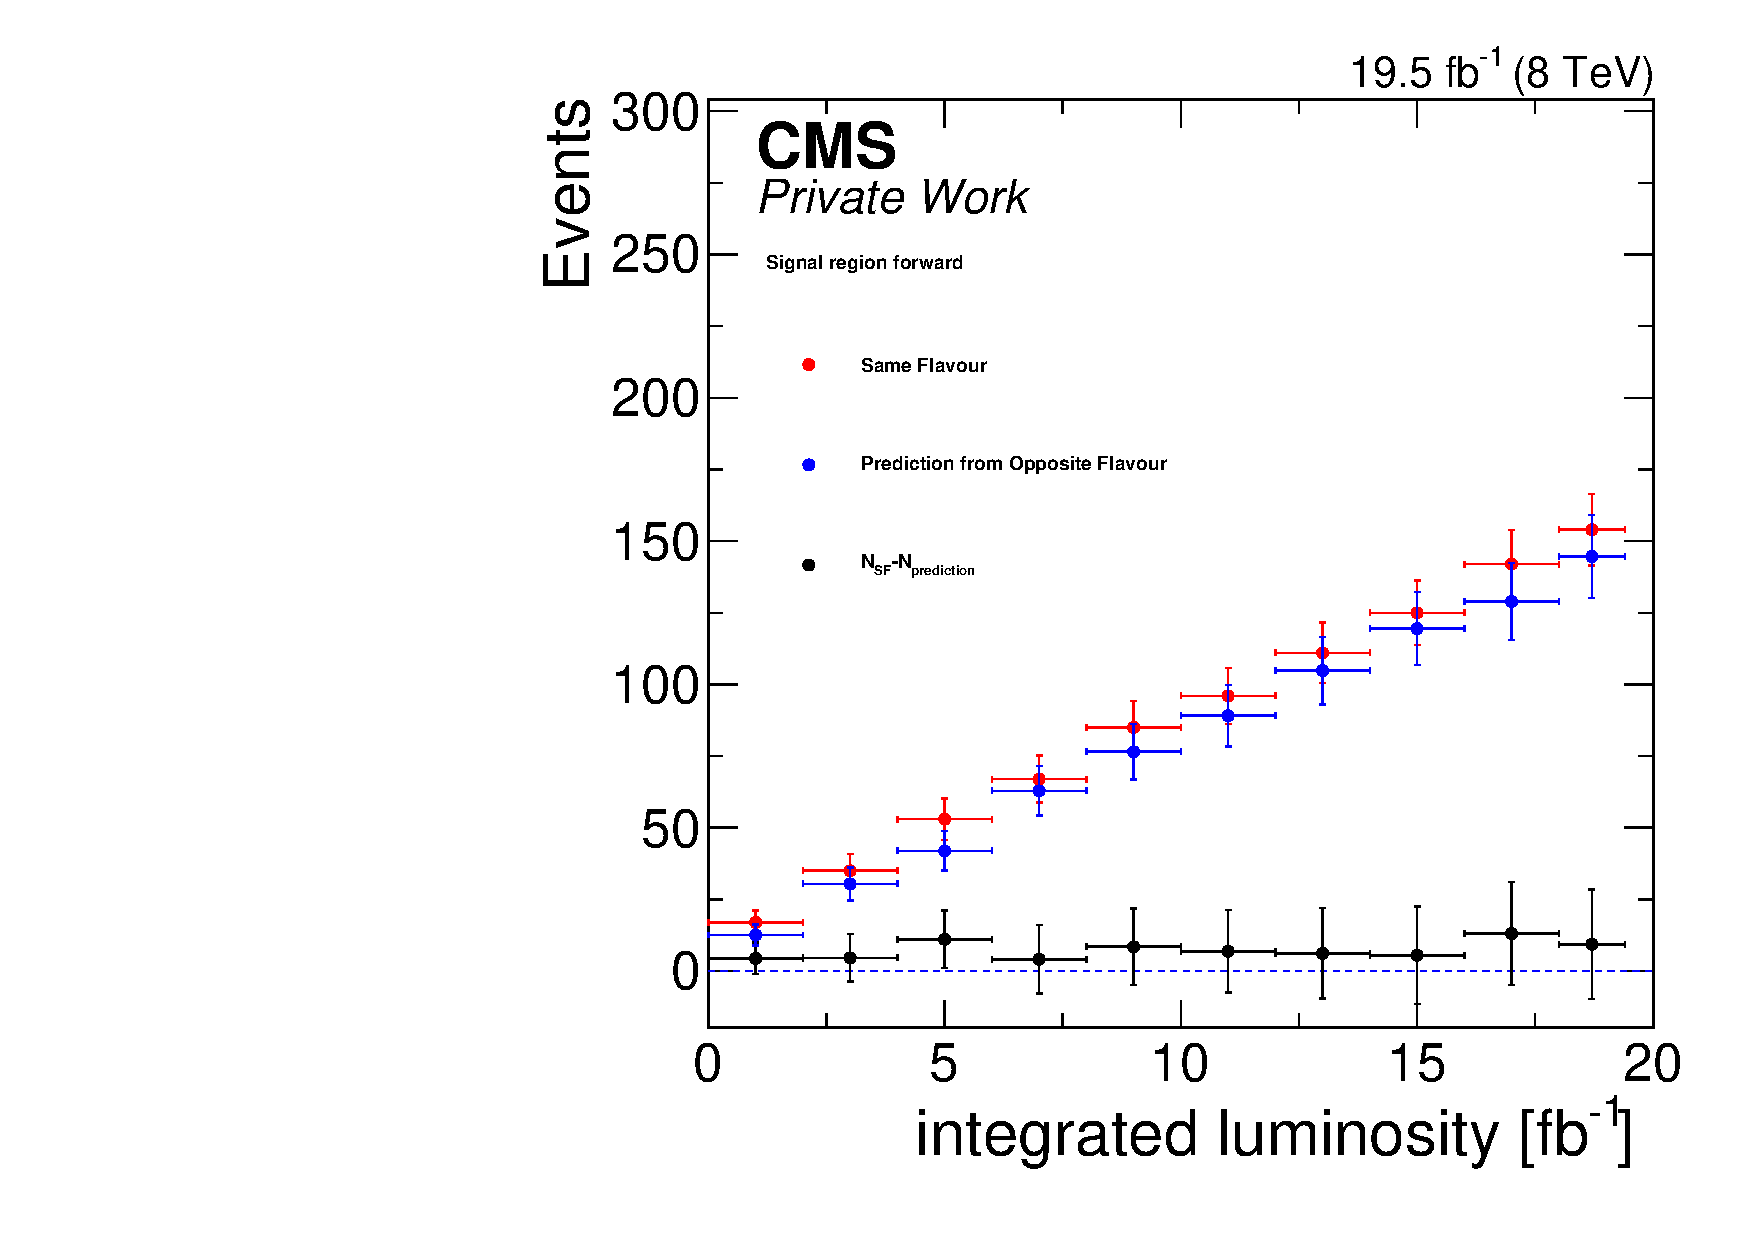
\includegraphics[width=\textwidth]{plots/results/YieldvsLumi_SignalForward_Mll_edgeMassFull2012.pdf}
\end{minipage}

\caption{Distribution of \mll in the signal region for the central (left) and forward (right) dilepton selection. The data is shown as black dots, while the total background prediction from data is shown as a blue histogram. The blue error bars indicate the combined statistical and systematic background uncertainty in each bin. The contribution from backgrounds containing a Z boson is shown as a green histogram. The dashed lines indicates the boundaries of the three mass bins. Beneath the plot the ratio of data to the background prediction is shown. The error bars include the statistical uncertainties of data and background, while the blue band indicates the systematic uncertainties on the background. }
\label{fig:timeDependece}
\end{figure}





\begin{table}[hbtp]
 \renewcommand{\arraystretch}{1.3}
 \setlength{\belowcaptionskip}{6pt}
 \centering
 \caption{Results of the counting experiment in the low-mass central signal region for different variations of the event selection. The observed event yield in SF events is compared with the combined estimate from flavour-symmetric and Drell--Yan backgrounds. The estimate for the Drell--Yan backgrounds is obtained by extrapolating the event yield in the on-Z signal region after subtraction of flavour-symmetric backgrounds to the low-mass region using the \Routin factor.}
  \label{tab:CountingCrosschecks}
  \begin{tabular}{l|c|c|c|c}
                                &  SF        & Flavour-symmetric  &  Drell--Yan  & Observed - Estimates \\ 

    \hline
    \hline
 & \multicolumn{4}{c}{b-tagging}\\ 
\hline 
        no b-tags       &  202                   & 188.5$\pm$15.4              &  7.1$\pm$2.5            &  6.3$\pm$21.1 \\
        $\geq$ 1 b-tags       &  663                   & 558.4$\pm$31.0              &  1.9$\pm$0.7            &  102.7$\pm$40.3 \\
\hline 
 & \multicolumn{4}{c}{lepton \pt requirement} \\ 
\hline 
        \pt > 20(10)\GeV       &  1474                   & 1290.2$\pm$58.6              &  11.4$\pm$4.1            &  172.5$\pm$70.1 \\
        \pt > 30(10)\GeV       &  1262                   & 1114.8$\pm$52.1              &  11.3$\pm$4.1            &  135.9$\pm$63.2 \\
        \pt > 30(20)\GeV       &  761                   & 674.0$\pm$35.5              &  9.0$\pm$3.3            &  78.0$\pm$45.1 \\
        \pt > 30\GeV       &  296                   & 275.7$\pm$19.4              &  6.5$\pm$2.3            &  13.8$\pm$26.0 \\
\hline 
 & \multicolumn{4}{c}{tight lepton isolation} \\ 
\hline 
        rel. isolation < 0.05       &  572                   & 491.5$\pm$28.4              &  7.1$\pm$2.6            &  73.3$\pm$37.2 \\
\hline 
 & \multicolumn{4}{c}{pileup} \\ 
\hline 
        $N_{\text{vtx}} <$ 13       &  332                   & 289.9$\pm$20.0              &  3.3$\pm$1.2            &  38.8$\pm$27.1 \\
        13 $\leq N_{\text{vtx}}$ < 17       &  242                   & 212.8$\pm$16.5              &  0.9$\pm$0.3            &  28.3$\pm$22.7 \\
        $N_{\text{vtx}} \geq$ 17       &  291                   & 244.2$\pm$18.0              &  4.8$\pm$1.7            &  41.9$\pm$24.8 \\
\hline 
 & \multicolumn{4}{c}{\MET reconstructions}\\
\hline 
        type I corrected PF \MET       &  1034                   & 923.3$\pm$45.0              &  9.4$\pm$3.4            &  101.3$\pm$55.4 \\
        track corrected \MET       &  850                   & 702.3$\pm$36.6              &  26.3$\pm$9.4            &  121.3$\pm$47.7 \\
        missing $H_{\mathrm{T}}$       &  1171                   & 942.5$\pm$45.7              &  50.8$\pm$18.1            &  177.6$\pm$59.9 \\
\hline 
 & \multicolumn{4}{c}{$H_{\mathrm{T}}$}\\
\hline 
        100\GeV $< H_{\mathrm{T}} < $ 300\GeV        &  455                   & 401.3$\pm$24.7              &  1.4$\pm$0.5            &  52.3$\pm$32.7 \\
        $H_{\mathrm{T}} > $ 300\GeV        &  410                   & 344.6$\pm$22.4              &  7.5$\pm$2.7            &  57.9$\pm$30.3 \\
\hline 


  \end{tabular}
\end{table}





\begin{figure}[htbp]
\centering
\begin{minipage}[t]{0.49\textwidth}
  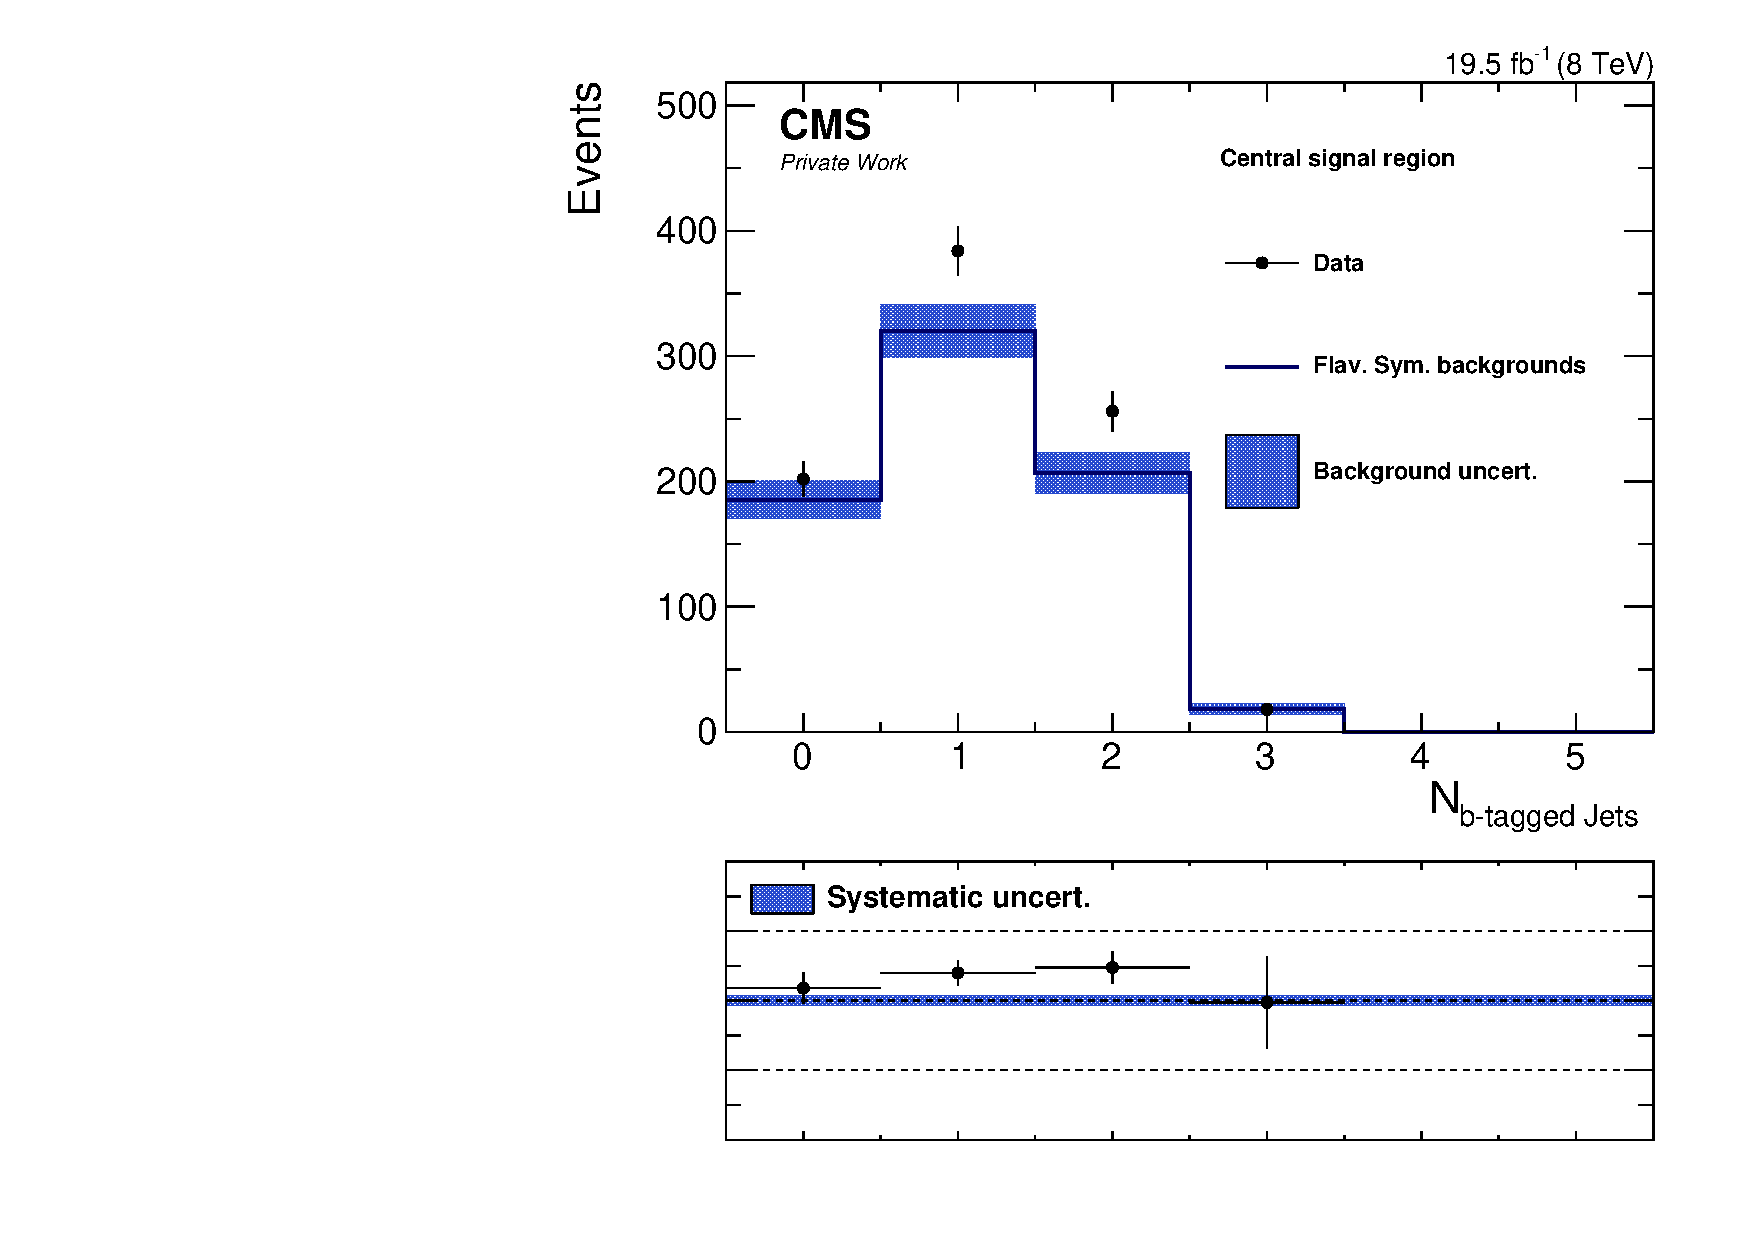
\includegraphics[width=\textwidth]{plots/results/rSFOFDependencies/rSFOFDependency_SignalCentral_NBJets_Full2012_SF_lowMass.pdf}
\end{minipage}
\begin{minipage}[t]{0.49\textwidth}
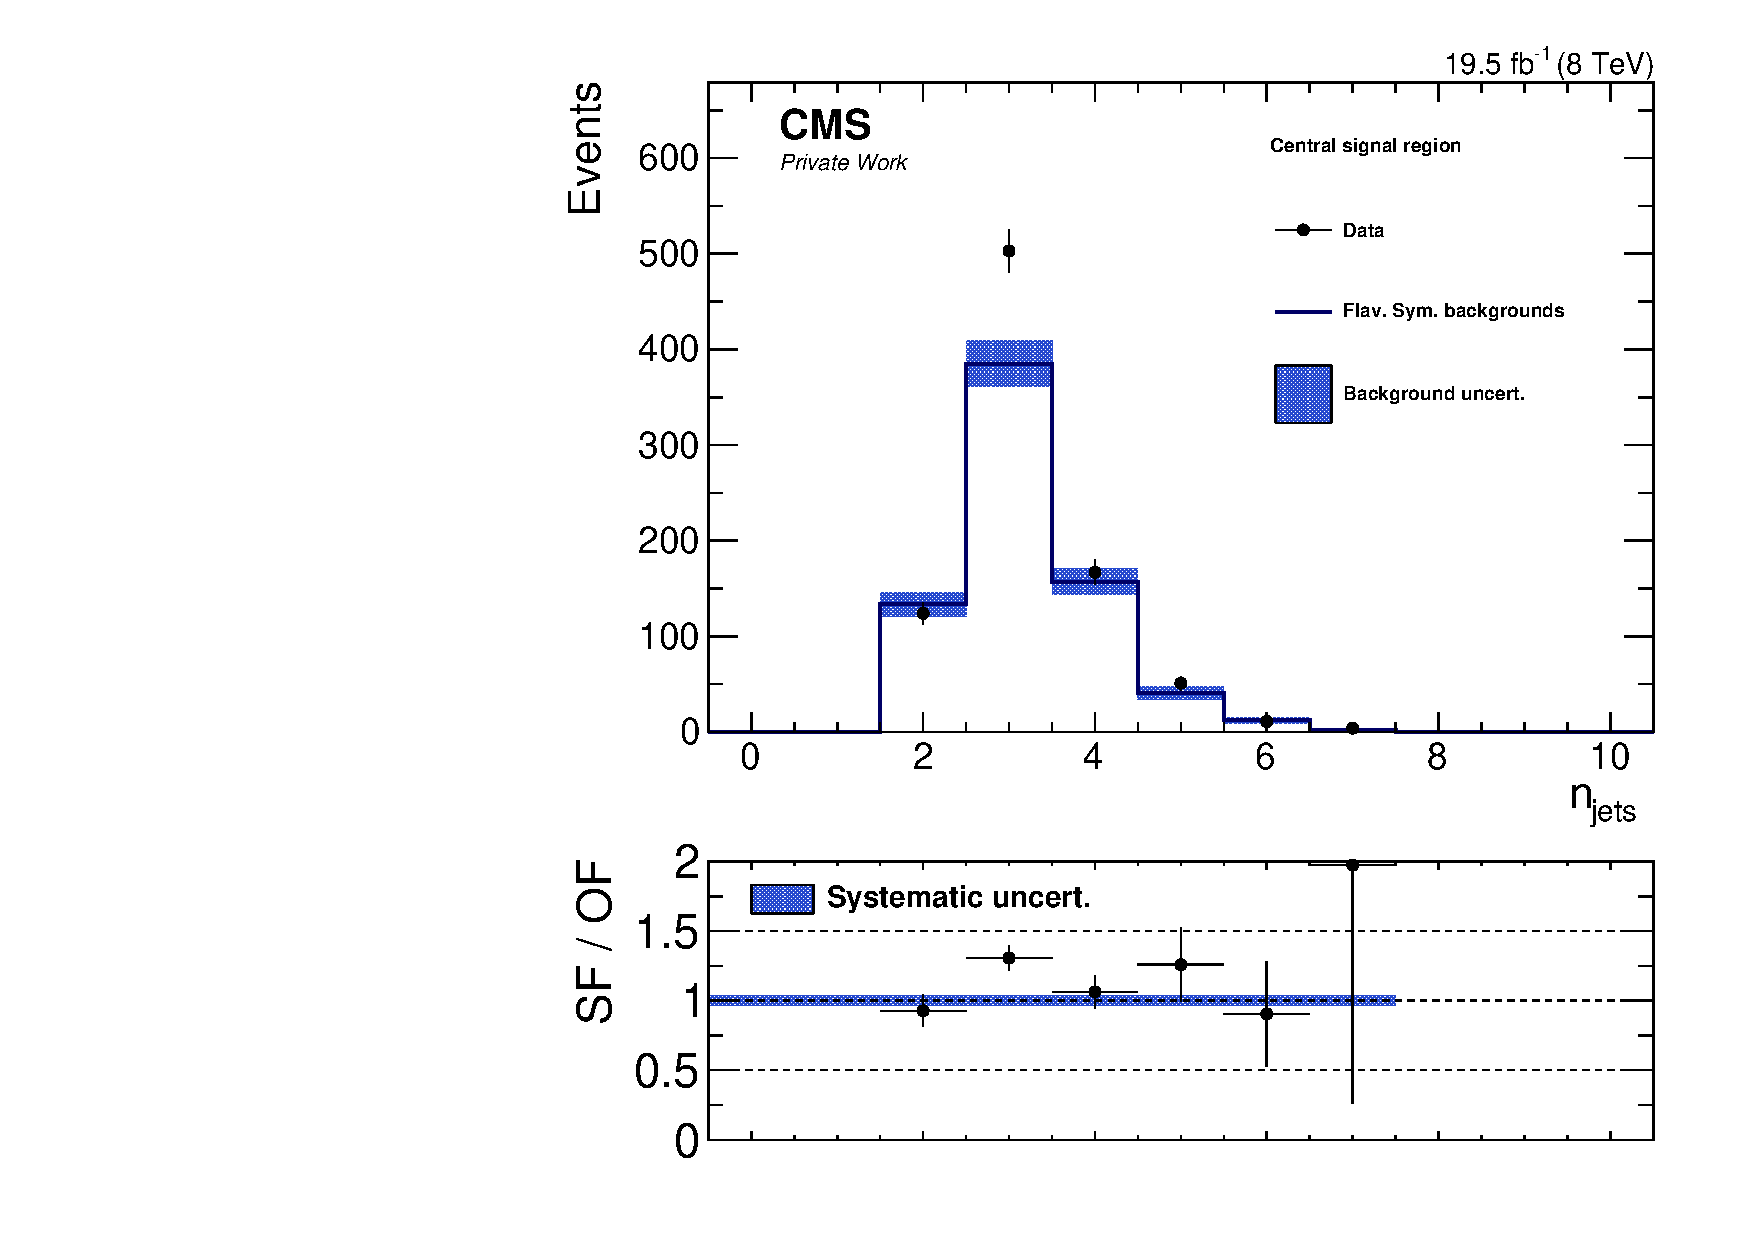
\includegraphics[width=\textwidth]{plots/results/rSFOFDependencies/rSFOFDependency_SignalCentral_NJets_Full2012_SF_lowMass.pdf}
\end{minipage}
\begin{minipage}[t]{0.49\textwidth}
  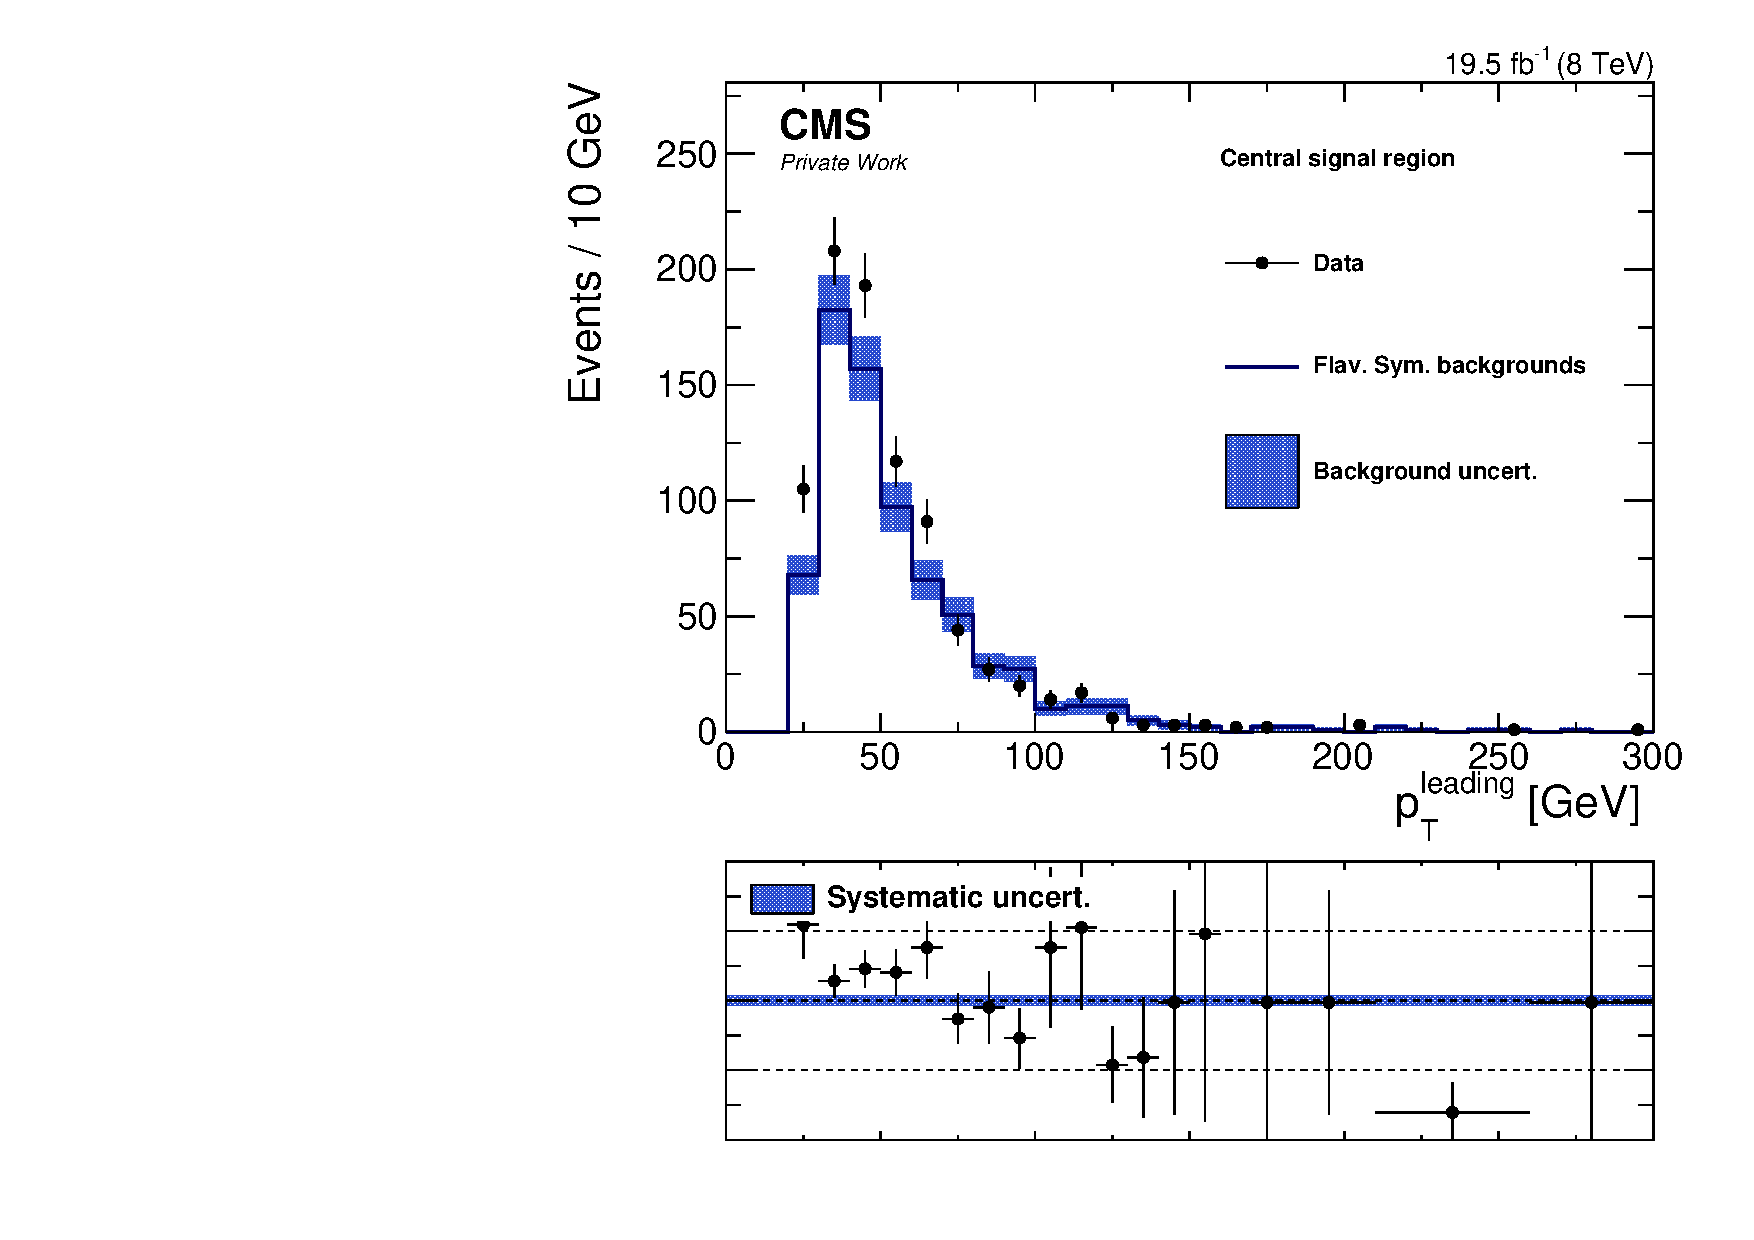
\includegraphics[width=\textwidth]{plots/results/rSFOFDependencies/rSFOFDependency_SignalCentral_LeadingPt_Full2012_SF_lowMass.pdf}
\end{minipage}
\begin{minipage}[t]{0.49\textwidth}
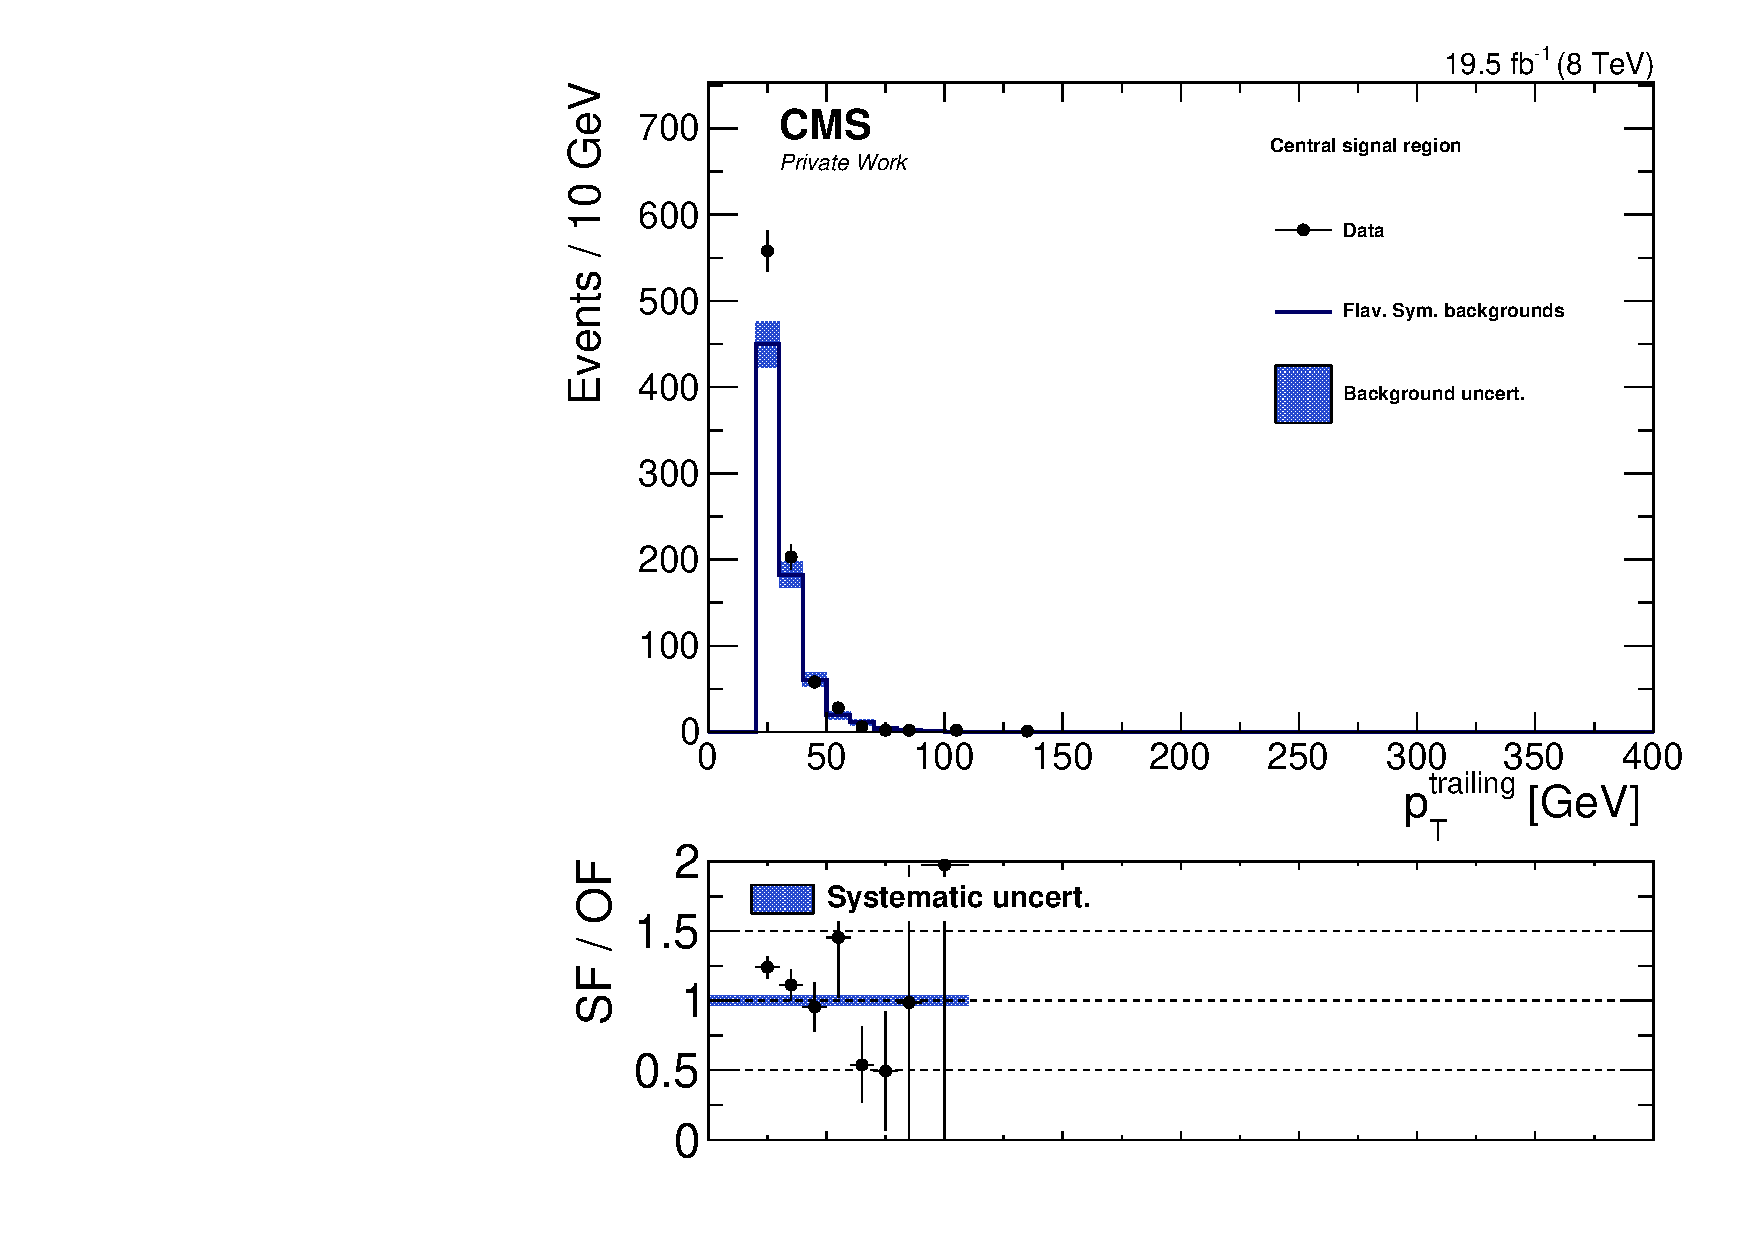
\includegraphics[width=\textwidth]{plots/results/rSFOFDependencies/rSFOFDependency_SignalCentral_TrailingPt_Full2012_SF_lowMass.pdf}
\end{minipage}
\begin{minipage}[t]{0.49\textwidth}
  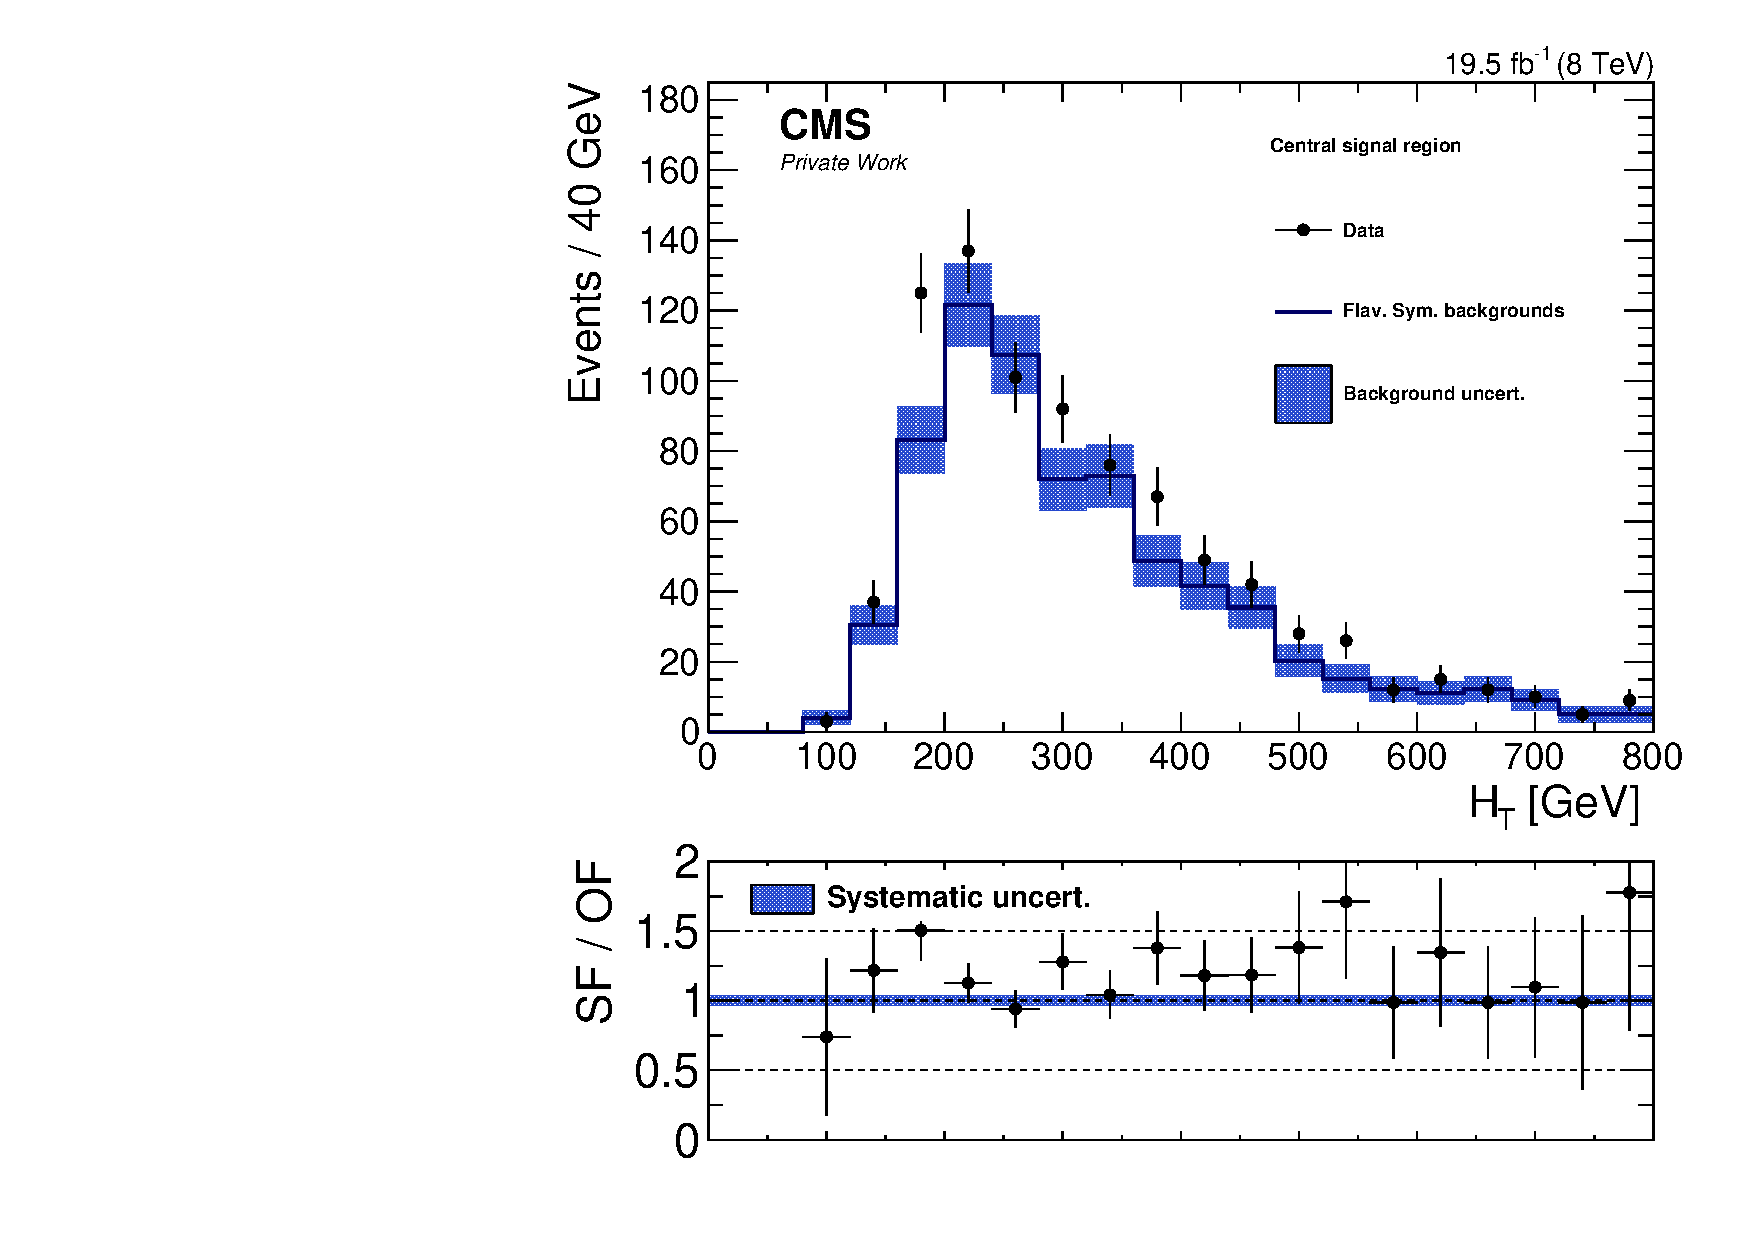
\includegraphics[width=\textwidth]{plots/results/rSFOFDependencies/rSFOFDependency_SignalCentral_HT_Full2012_SF_lowMass.pdf}
\end{minipage}
\begin{minipage}[t]{0.49\textwidth}
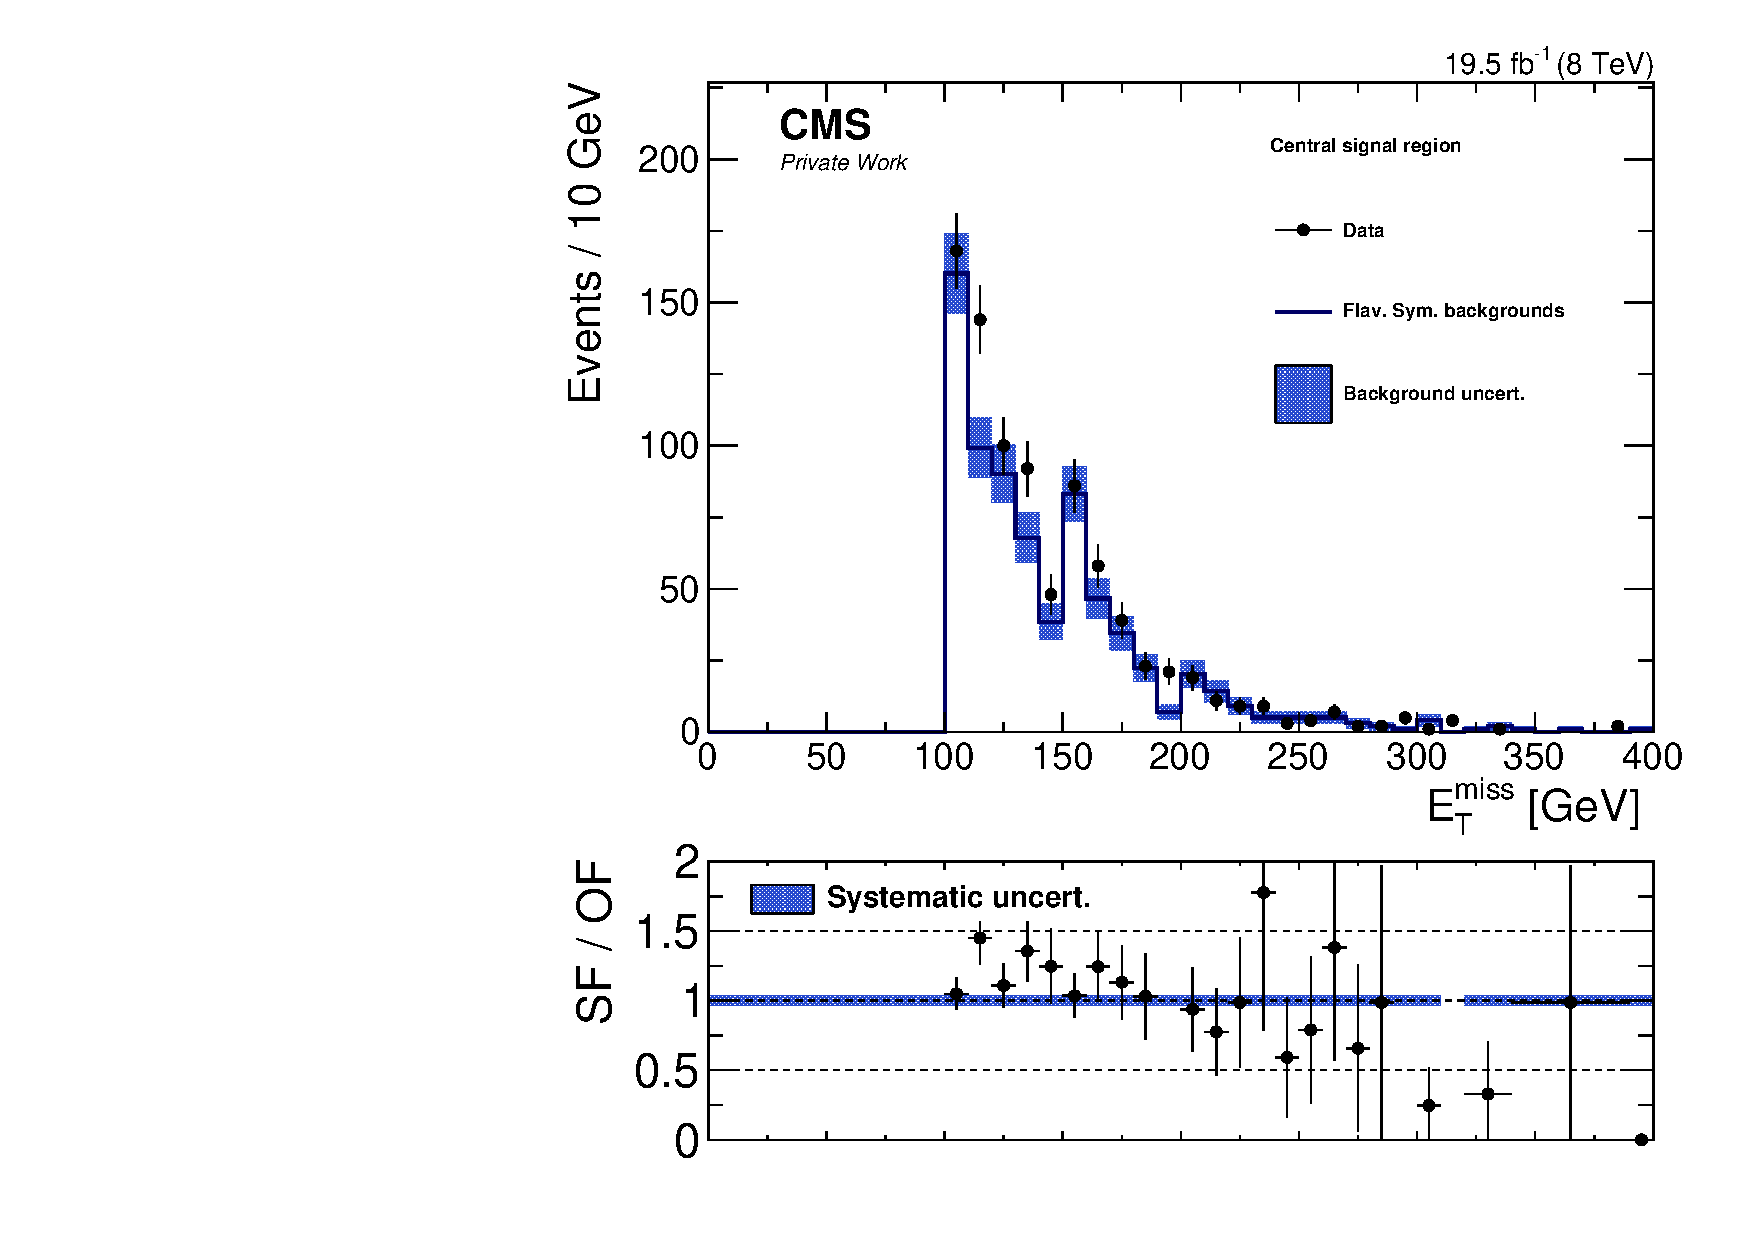
\includegraphics[width=\textwidth]{plots/results/rSFOFDependencies/rSFOFDependency_SignalCentral_MET_Full2012_SF_lowMass.pdf}
\end{minipage}
\caption{Distribution of \mll in the signal region for the central (left) and forward (right) dilepton selection. The data is shown as black dots, while the total background prediction from data is shown as a blue histogram. The blue error bars indicate the combined statistical and systematic background uncertainty in each bin. The contribution from backgrounds containing a Z boson is shown as a green histogram. The dashed lines indicates the boundaries of the three mass bins. Beneath the plot the ratio of data to the background prediction is shown. The error bars include the statistical uncertainties of data and background, while the blue band indicates the systematic uncertainties on the background. }
\label{fig:timeDependece}
\end{figure}


\section{Result of the search for a kinematic edge}